\documentclass[11pt]{article}
\usepackage{worksheet_style}

% ---- Toggle: uncomment for filled version ----
%\worksheetfilledtrue
\begin{document}
\worksheetheader{18}{Applications of Multiple Integrals}

\begin{background}
Now that we can integrate over general regions, we put multiple integrals to work. Mass, center of mass, moments of inertia, and average value all reduce to integrals with the right integrand --- the same recipe in 2D and in 3D. We also derive the surface area formula, extending arc length to two dimensions.
\end{background}

%=============================================================
\wsection{Warm-Up: Double Integral Review}

Evaluate $\ds\int_0^1\int_0^{1-x} (x+y)\,dy\,dx$.

1. Inner integral ($y$): $\ds\int_0^{1-x}(x+y)\,dy = \wbml{\left[xy + \frac{y^2}{2}\right]_0^{1-x} = x(1-x)+\frac{(1-x)^2}{2}}$

2. Simplify: $\wbml{x - x^2 + \frac{1-2x+x^2}{2} = \frac{1}{2} - \frac{x^2}{2}}$

3. Outer integral: $\ds\int_0^1 \left(\frac{1}{2}-\frac{x^2}{2}\right)dx = \wbml{\left[\frac{x}{2}-\frac{x^3}{6}\right]_0^1 = \frac{1}{2}-\frac{1}{6} = \boxed{\frac{1}{3}}}$

%=============================================================
\wsection{Mass and Center of Mass}

\begin{formulabox}{Mass, Moments, and Center of Mass}
For a lamina with density $\rho(x,y)$ over region $R$:
\begin{align*}
\text{Mass:} \quad M &= \iint_R \rho(x,y)\,dA \\[4pt]
\text{Moments:} \quad M_x &= \iint_R y\,\rho(x,y)\,dA \quad \text{(about $x$-axis)} \\
M_y &= \iint_R x\,\rho(x,y)\,dA \quad \text{(about $y$-axis)} \\[4pt]
\text{Center of mass:} \quad \bar{x} &= \frac{M_y}{M}, \qquad \bar{y} = \frac{M_x}{M}
\end{align*}
-- $M_x$ uses $y$ (distance to $x$-axis); $M_y$ uses $x$ (distance to $y$-axis)

-- If $\rho = $ const, center of mass $=$ centroid
\end{formulabox}

\begin{center}
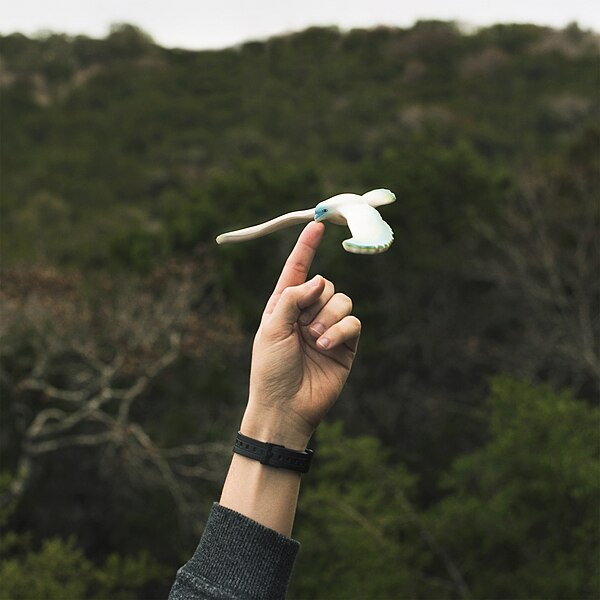
\includegraphics[width=5cm]{pics/COG.jpg}\\
{\small Center of mass of a system of point masses.}
\end{center}

\begin{example}[Center of Mass of a Triangular Lamina]
Find the mass and center of mass of a triangular lamina with vertices $(0,0)$, $(2,0)$, $(0,1)$ and density $\rho(x,y) = 1+x$.

\wbbox{
1. \textbf{Region (Type I):} $0 \le x \le 2$, $0 \le y \le 1 - x/2$.

2. \textbf{Mass:}
$M = \int_0^2\int_0^{1-x/2}(1+x)\,dy\,dx = \int_0^2 (1+x)(1-x/2)\,dx$

$= \int_0^2\left(1+\frac{x}{2}-\frac{x^2}{2}\right)dx = \left[x+\frac{x^2}{4}-\frac{x^3}{6}\right]_0^2 = 2+1-\frac{4}{3} = \frac{5}{3}$

3. \textbf{Moment $M_y$:}
$M_y = \int_0^2\int_0^{1-x/2}x(1+x)\,dy\,dx = \int_0^2 x(1+x)(1-x/2)\,dx$

$= \int_0^2\left(x+\frac{x^2}{2}-\frac{x^3}{2}\right)dx = \left[\frac{x^2}{2}+\frac{x^3}{6}-\frac{x^4}{8}\right]_0^2 = 2+\frac{4}{3}-2 = \frac{4}{3}$

4. \textbf{Moment $M_x$:}
$M_x = \int_0^2\int_0^{1-x/2}y(1+x)\,dy\,dx = \int_0^2 (1+x)\frac{(1-x/2)^2}{2}\,dx = \frac{5}{12}$

5. \textbf{Center of mass:}
$\bar{x} = \frac{M_y}{M} = \frac{4/3}{5/3} = \frac{4}{5}, \qquad \bar{y} = \frac{M_x}{M} = \frac{5/12}{5/3} = \frac{1}{4}$

6. \textbf{Result:} $\boxed{(\bar{x},\bar{y}) = \left(\frac{4}{5},\,\frac{1}{4}\right)}$

\textit{The center of mass shifts right because the density $1+x$ is heavier on the right.}
}{7cm}
\end{example}

%=============================================================
\wsection{Moments of Inertia}

\begin{formulabox}{Moments of Inertia}
\begin{align*}
I_x &= \iint_R y^2\,\rho\,dA \quad \text{(about the $x$-axis)} \\
I_y &= \iint_R x^2\,\rho\,dA \quad \text{(about the $y$-axis)} \\
I_z = I_0 &= \iint_R (x^2+y^2)\,\rho\,dA \quad \text{(polar moment / about the origin)}
\end{align*}
Note: $I_z = I_x + I_y$.

\medskip
\textbf{Physics connections:}
\begin{itemize}[nosep, leftmargin=*]
  \item Rotational kinetic energy: $KE = \frac{1}{2}I\omega^2$
  \item Newton's second law for rotation: $\tau = I\alpha$
\end{itemize}
\end{formulabox}

\begin{example}[DJ Turntable Platter]
A circular platter (annular disk, inner radius $R_1 = 1$, outer radius $R_2 = 2$) has density $\rho(r) = kr^2$ (denser at the rim). If total mass is $M = 1$ kg, find $k$ and the polar moment of inertia $I_z$.

\wbbox{
1. \textbf{Find $k$ from mass:}
$M = \int_0^{2\pi}\int_1^2 kr^2 \cdot r\,dr\,d\theta = 2\pi k\int_1^2 r^3\,dr = 2\pi k\left[\frac{r^4}{4}\right]_1^2 = 2\pi k\cdot\frac{15}{4} = \frac{15\pi k}{2}$

$\frac{15\pi k}{2} = 1 \implies k = \frac{2}{15\pi}$

2. \textbf{Polar moment of inertia:} $I_z = \iint (x^2+y^2)\rho\,dA = \iint r^2 \cdot kr^2 \cdot r\,dr\,d\theta$

$I_z = 2\pi k\int_1^2 r^5\,dr = 2\pi k\left[\frac{r^6}{6}\right]_1^2 = 2\pi k\cdot\frac{63}{6} = 21\pi k$

3. \textbf{Substitute $k$:}
$I_z = 21\pi\cdot\frac{2}{15\pi} = \frac{42}{15} = \frac{14}{5}$

4. \textbf{Result:} $\boxed{I_z = \frac{14}{5} \approx 2.8 \text{ kg}\cdot\text{m}^2}$

\textit{Compare: a uniform annular disk of the same mass has $I_z = \frac{1}{2}M(R_1^2+R_2^2) = 2.5$. The rim-heavy platter has a larger moment of inertia, as expected.}
}{7cm}
\end{example}

%=============================================================
\wsection{Surface Area}

\begin{thmbox}{Surface Area Formula}
The surface area of $z = f(x,y)$ over a region $R$ in the $xy$-plane:
\[A = \iint_R \sqrt{1 + \left(\frac{\partial f}{\partial x}\right)^2 + \left(\frac{\partial f}{\partial y}\right)^2}\,dA\]
-- This generalizes the arc length formula $\int\sqrt{1+(f')^2}\,dx$ to surfaces
\end{thmbox}

\begin{example}[Surface Area of a Paraboloid]
Find the surface area of $z = x^2 + y^2$ over the disk $x^2+y^2 \le 4$.

\wbbox{
1. \textbf{Partial derivatives:} $f_x = 2x$, $f_y = 2y$.

2. \textbf{Integrand:} $\sqrt{1+4x^2+4y^2} = \sqrt{1+4r^2}$ in polar.

3. \textbf{Set up (polar):}
$A = \int_0^{2\pi}\int_0^2 \sqrt{1+4r^2}\cdot r\,dr\,d\theta = 2\pi\int_0^2 r\sqrt{1+4r^2}\,dr$

4. \textbf{Substitution:} $u = 1+4r^2$, $du = 8r\,dr$, so $r\,dr = du/8$.

When $r=0$: $u=1$. When $r=2$: $u=17$.

$A = 2\pi\cdot\frac{1}{8}\int_1^{17}\sqrt{u}\,du = \frac{\pi}{4}\cdot\left[\frac{2}{3}u^{3/2}\right]_1^{17} = \frac{\pi}{6}(17\sqrt{17}-1)$

5. \textbf{Result:} $\boxed{A = \frac{\pi}{6}(17\sqrt{17}-1) \approx 36.2}$
}{5.5cm}
\end{example}

%=============================================================
\wsection{Applications via Triple Integrals}

\begin{formulabox}{Mass, Center of Mass, and Moments of Inertia in 3D}
For a solid $E$ with density $\rho(x,y,z)$:
\begin{align*}
\text{Mass:} \quad M &= \iiint_E \rho\,dV \\[4pt]
\text{Center of mass:} \quad \bar{x} &= \frac{1}{M}\iiint_E x\,\rho\,dV, \quad \bar{y} = \frac{1}{M}\iiint_E y\,\rho\,dV, \quad \bar{z} = \frac{1}{M}\iiint_E z\,\rho\,dV \\[4pt]
\text{Moments of inertia:} \quad I_x &= \iiint_E (y^2+z^2)\,\rho\,dV \\
I_y &= \iiint_E (x^2+z^2)\,\rho\,dV \\
I_z &= \iiint_E (x^2+y^2)\,\rho\,dV
\end{align*}
-- $I_x$ uses $y^2+z^2$ --- the squared distance from the $x$-axis. Same pattern for $I_y$ and $I_z$.

-- Rotational kinetic energy about the $z$-axis: $KE = \tfrac{1}{2} I_z\,\omega^2$.
\end{formulabox}

\begin{example}[Center of Mass of a Solid Tetrahedron]
A solid tetrahedron $E$ has vertices $(0,0,0)$, $(1,0,0)$, $(0,1,0)$, $(0,0,1)$ and uniform density $\rho = 1$. Find its center of mass.

\wbbox{
1. \textbf{Region:} $0 \le z \le 1-x-y$, $0 \le y \le 1-x$, $0 \le x \le 1$.

2. \textbf{Mass:}
$M = \int_0^1\!\!\int_0^{1-x}\!\!\int_0^{1-x-y} 1\,dz\,dy\,dx = \int_0^1\!\!\int_0^{1-x}(1-x-y)\,dy\,dx = \int_0^1 \tfrac{(1-x)^2}{2}\,dx = \tfrac{1}{6}$.

3. \textbf{Moment about the $yz$-plane:}
$\iiint_E x\,dV = \int_0^1\!\!\int_0^{1-x}\!\!\int_0^{1-x-y} x\,dz\,dy\,dx = \int_0^1 x\cdot\tfrac{(1-x)^2}{2}\,dx = \tfrac{1}{24}$.

So $\bar{x} = \dfrac{1/24}{1/6} = \tfrac{1}{4}$.

4. By symmetry of the tetrahedron and density, $\bar{y} = \bar{z} = \tfrac{1}{4}$.

5. \textbf{Result:} $\boxed{(\bar{x},\bar{y},\bar{z}) = \left(\tfrac{1}{4},\,\tfrac{1}{4},\,\tfrac{1}{4}\right)}$ --- the centroid sits one-quarter of the way along each axis.
}{7cm}
\end{example}

\begin{example}[Moment of Inertia of a Solid Cylinder]
A solid cylinder $E$ of radius $R$ and height $h$ sits along the $z$-axis with uniform density $\rho_0$. Find $I_z$ in terms of the total mass $M = \pi R^2 h\,\rho_0$.

\wbbox{
1. \textbf{Cylindrical coordinates:} $0 \le r \le R$, $0 \le \theta \le 2\pi$, $0 \le z \le h$, $dV = r\,dr\,d\theta\,dz$.

2. \textbf{Set up:}
$I_z = \iiint_E (x^2+y^2)\rho_0\,dV = \rho_0\int_0^h\!\!\int_0^{2\pi}\!\!\int_0^R r^2\cdot r\,dr\,d\theta\,dz = \rho_0\cdot h\cdot 2\pi\cdot\tfrac{R^4}{4}$.

3. \textbf{Simplify:}
$I_z = \tfrac{\pi R^4 h\,\rho_0}{2} = \tfrac{1}{2}MR^2$.

4. \textbf{Result:} $\boxed{I_z = \tfrac{1}{2}MR^2}$ --- the standard result for a uniform solid cylinder.
}{5cm}
\end{example}

%=============================================================
\wsection{Average Value}

\begin{formulabox}{Average Value of a Function}
The average value of $f$ over a region is its integral divided by the size of the region:
\begin{align*}
\text{2D:} \quad \bar f &= \frac{1}{\text{Area}(R)} \iint_R f\,dA \\[2pt]
\text{3D:} \quad \bar f &= \frac{1}{\text{Vol}(E)} \iiint_E f\,dV
\end{align*}
-- Same idea as $\bar f = \tfrac{1}{b-a}\int_a^b f(x)\,dx$ from Calc I.
\end{formulabox}

\begin{example}[Average Temperature in a Cube]
The unit cube $E = [0,1]^3$ has temperature $T(x,y,z) = x+y+z$. Find the average temperature.

\wbbox{
1. \textbf{Volume:} $\text{Vol}(E) = 1$.

2. \textbf{Integrate:}
$\iiint_E (x+y+z)\,dV = \int_0^1\!\!\int_0^1\!\!\int_0^1(x+y+z)\,dz\,dy\,dx$.

By symmetry, $\iiint_E x\,dV = \iiint_E y\,dV = \iiint_E z\,dV = \tfrac{1}{2}$, so the sum is $\tfrac{3}{2}$.

3. \textbf{Result:} $\bar T = \dfrac{3/2}{1} = \boxed{\tfrac{3}{2}}$ --- exactly the value of $T$ at the center $(\tfrac{1}{2},\tfrac{1}{2},\tfrac{1}{2})$, which makes sense because $T$ is linear.
}{4.5cm}
\end{example}

%=============================================================

\begin{practice}

\prob Find the mass of a lamina over $R = [0,1]\times[0,2]$ with density $\rho(x,y) = xy$.

\wans{\wbm{$M = 1$}}

\vspace{3cm}

\prob Find $I_z$ for a uniform disk of radius $R$ with constant density $\rho_0$. Express in terms of the total mass $M = \pi R^2\rho_0$.

\wans{\wbml{$I_z = \frac{1}{2}MR^2$}}

\vspace{4cm}

\prob A disk of radius 2 has density $\rho = 4-x^2-y^2$. A torque of $\tau = 12$ N$\cdot$m is applied. Find the angular acceleration $\alpha = \tau/I_z$.

\wans{\wbml{$I_z = 32\pi/3$, so $\alpha = 9/(8\pi) \approx 0.358$ rad/s$^2$}}

\vspace{5cm}

\prob Find the center of mass of the region bounded by $y = x^2$ and $y = 4$ with uniform density $\rho = 1$.

\wans{\wbml{$(\bar{x}, \bar{y}) = (0, 12/5)$}}

\vspace{5cm}

\prob Set up (do not evaluate) the surface area integral for $z = e^{x}\sin y$ over the rectangle $[0,1]\times[0,\pi]$.

\wans{\wbml{$A = \int_0^1\int_0^\pi \sqrt{1+e^{2x}\sin^2 y + e^{2x}\cos^2 y}\,dy\,dx = \int_0^1\int_0^\pi\sqrt{1+e^{2x}}\,dy\,dx$}}

\vspace{3cm}

\prob Find the mass of the solid box $E = [0,1]\times[0,2]\times[0,3]$ with density $\rho(x,y,z) = xyz$.

\wans{\wbml{$M = \int_0^1\int_0^2\int_0^3 xyz\,dz\,dy\,dx = \tfrac{1}{2}\cdot 2\cdot \tfrac{9}{2} = \tfrac{9}{2}$}}

\vspace{3cm}

\prob A solid cone of radius $R$ and height $h$ has uniform density $\rho_0$ and total mass $M=\tfrac{1}{3}\pi R^2 h\,\rho_0$. Find its moment of inertia $I_z$ about the central axis. \textit{Hint: cylindrical coordinates with $0 \le r \le Rz/h$.}

\wans{\wbml{$I_z = \tfrac{3}{10}MR^2$}}

\vspace{4cm}

\prob Find the average value of $f(x,y,z) = x^2+y^2+z^2$ over the unit ball $x^2+y^2+z^2 \le 1$. \textit{Hint: spherical coordinates; $\text{Vol}=\tfrac{4\pi}{3}$.}

\wans{\wbml{$\iiint_E \rho^2\cdot \rho^2\sin\phi\,d\rho\,d\phi\,d\theta = \tfrac{4\pi}{5}$, so $\bar f = \dfrac{4\pi/5}{4\pi/3} = \tfrac{3}{5}$}}

\vspace{4cm}

\end{practice}

\end{document}
